\documentclass[aspectratio=169]{beamer}
\usepackage[utf8]{inputenc}
\usepackage[T1]{fontenc}
\usepackage{lmodern}
\usepackage[brazil]{babel}

% Caso não tenha o tema DCC no seu ambiente, pode usar \usetheme{Madrid}
\usetheme{DCC}
\setbeamertemplate{itemize items}[circle]
\setlength{\parskip}{0.5em}
\graphicspath{{imgs/}, {./}} % Busca imagens na pasta imgs/ ou na raiz

% Protege o conteúdo da faixa lateral
\setbeamersize{text margin left=1cm,text margin right=0.6cm}

% Convenções de formatação:
%   \textit{...} -> termos em inglês (Extension Host, thread, zero-copy...)
%   \texttt{...} -> código, arquivos e identificadores (libobs, obs-module.h...)
%   \fonte{...}  -> apenas em conteúdo de fonte externa ou figura própria

\author[Felipe, Jaedson, Lucas, Nadson]{%
\textbf{Felipe Silva da Anunciação}\\[0.12cm]
\textbf{Jaedson Barbosa Macedo}\\[0.12cm]
\textbf{Lucas Pereira Rapozo}\\[0.12cm]
\textbf{Nadson de Santana Sousa}}

\title{Estilo Arquitetural Microkernel\\Análise: VS Code e OBS Studio}
\institute{Universidade Federal da Bahia (UFBA)\\
Engenharia de Software I --- MATA62 -- T01 --- Equipe 03\\
Docente: Prof. Dr. Eduardo Almeida}
\date{Salvador, 2026}

\newcommand{\fonte}[1]{\par\vspace{0.12cm}{\scriptsize\color{gray}Fonte: #1}}

\begin{document}

\begin{frame}[plain,noframenumbering]
\titlepage
\end{frame}

% ==========================================================
% O ESTILO MICROKERNEL
% ==========================================================

\begin{frame}{O Estilo Microkernel}
\begin{itemize}\setlength{\itemsep}{0.65em}
\item Este padrão é também conhecido como Arquitetura Baseada em Plugins (\textit{Plugin-Based Architecture}).
\item Resolve a necessidade de adicionar novas funcionalidades sem causar degradação estrutural no núcleo do sistema.
\item Permite evitar a formação do antipadrão arquitetural \textit{Big Ball of Mud} ao longo do tempo.
\item \textbf{Estrutura Central:} É composta por um \textit{Core System} (sistema central) enxuto e múltiplos \textit{Plug-in Components} acopláveis de forma independente.
\item Promove um forte desacoplamento e facilita consideravelmente a manutenção a longo prazo.
\end{itemize}
\fonte{Richards e Ford (2020).}
\end{frame}

% ==========================================================
% VISUAL STUDIO CODE
% ==========================================================

\begin{frame}{Visual Studio Code: Características Gerais}
No VS Code, identificaram-se as seguintes características arquiteturais:
\begin{itemize}\setlength{\itemsep}{0.4em}
\item \textbf{Extensibilidade, Desempenho e Confiabilidade:} Fundamentais para a fluidez e a estabilidade da ferramenta.
\item \textbf{Manutenibilidade e Modularidade:} Camadas com regras de dependência e injeção de dependências.
\item \textbf{Portabilidade:} A mesma base de código atende Windows, Linux, macOS e a versão web.
\item \textbf{Interoperabilidade e Reutilização:} Integração com ferramentas externas via protocolos abertos (LSP e DAP).
\item \textbf{Segurança e Configurabilidade:} \textit{Workspace Trust} para projetos não confiáveis e configurações em camadas.
\item \textbf{Agilidade, Testabilidade e Acessibilidade:} Lançamentos regulares, testes automatizados e suporte a leitores de tela.
\end{itemize}
\end{frame}

\begin{frame}{Visual Studio Code: Principais Características (Top 4) (1/2)}
\begin{itemize}\setlength{\itemsep}{0.8em}
\item \textbf{Extensibilidade (ADR-001):}
  \begin{itemize}
  \item É a razão de ser do estilo Microkernel neste sistema.
  \item Funcionalidades padrão, como Git e TypeScript, são entregues como extensões embarcadas.
  \item A própria Microsoft utiliza a mesma API pública oferecida a terceiros.
  \end{itemize}
\item \textbf{Confiabilidade e Tolerância a Falhas (ADR-002):}
  \begin{itemize}
  \item O sistema executa código de milhares de autores, sem garantia de qualidade, o que tornou obrigatório proteger o núcleo.
  \item Justificou o isolamento das extensões no \textit{Extension Host} (ADR-IMP-002): falhas em plugins não encerram o editor.
  \end{itemize}
\end{itemize}
\end{frame}

\begin{frame}{Visual Studio Code: Principais Características (Top 4) (2/2)}
\begin{itemize}\setlength{\itemsep}{0.8em}
\item \textbf{Desempenho (\textit{Performance}) (ADR-003):}
  \begin{itemize}
  \item Um editor de código precisa parecer leve: uma extensão lenta não pode travar a digitação.
  \item Motivou a ativação sob demanda das extensões (\textit{Activation Events}) e a comunicação assíncrona com o \textit{Extension Host}.
  \end{itemize}
\item \textbf{Interoperabilidade e Reutilização (ADR-004):}
  \begin{itemize}
  \item O editor precisa integrar ferramentas de diferentes linguagens e ecossistemas.
  \item Justificou a adoção do LSP e do DAP (ADR-IMP-003), permitindo reutilizar servidores de linguagem e adaptadores de depuração em outros editores.
  \end{itemize}
\end{itemize}
\end{frame}

\begin{frame}{Visual Studio Code: Características Fora do Top 4}
\begin{itemize}\setlength{\itemsep}{0.8em}
\item \textbf{Portabilidade:}
  \begin{itemize}
  \item Atendida sobretudo por decisões de tecnologia e de ambiente de execução (Electron, Node.js e navegador).
  \item É importante para distribuir o produto, mas não é a principal motivadora da estrutura Microkernel.
  \end{itemize}
\item \textbf{Segurança:}
  \begin{itemize}
  \item Tratada por mecanismos aplicados sobre a arquitetura já definida, como \textit{sandboxing}, \textit{Workspace Trust} e \textit{Restricted Mode}.
  \item Reduz riscos, mas não é o principal motivo da separação entre núcleo e extensões.
  \end{itemize}
\end{itemize}
\end{frame}

\begin{frame}{Visual Studio Code: Decisões Arquiteturais (ADRs) (1/2)}
\begin{itemize}\setlength{\itemsep}{0.8em}
\item \textbf{ADR-IMP-001: Adoção da Arquitetura Baseada em Plugins (Microkernel)}
  \begin{itemize}
  \item \textbf{Decisão:} Utilizar um sistema central aliado a múltiplos plugins acopláveis.
  \item \textbf{Consequências:} Promove um forte desacoplamento, facilita a manutenção a longo prazo e define um vocabulário claro de componentes.
  \end{itemize}
\item \textbf{ADR-IMP-002: Isolamento de Extensões via \textit{Extension Host}}
  \begin{itemize}
  \item \textbf{Decisão:} Executar o código de customização em um processo separado, que se comunica com o núcleo por chamadas remotas ou eventos assíncronos.
  \item \textbf{Consequências:} Falhas em plugins não derrubam a interface gráfica, ao custo da latência da comunicação entre processos (IPC).
  \end{itemize}
\end{itemize}
\end{frame}

\begin{frame}{Visual Studio Code: Decisões Arquiteturais (ADRs) (2/2)}
\begin{itemize}\setlength{\itemsep}{0.8em}
\item \textbf{ADR-IMP-003: Implementação do \textit{Language Server Protocol} (LSP)}
  \begin{itemize}
  \item \textbf{Decisão:} Utilizar o particionamento de domínio para delegar a análise sintática de código a servidores de linguagem que se comunicam de forma padronizada.
  \item \textbf{Consequências:} Aumenta a reutilização, pois o mesmo servidor de linguagem pode ser usado em outras ferramentas.
  \end{itemize}
\item \textbf{ADR-IMP-004: Utilização do framework Electron}
  \begin{itemize}
  \item \textbf{Decisão:} Encapsular tecnologias web (HTML/JS/CSS) usando o Electron como casca (\textit{wrapper}) da aplicação \textit{desktop}.
  \item \textbf{Consequências:} Reduz radicalmente a necessidade de múltiplas equipes de desenvolvimento nativo, em troca de um maior consumo de recursos da máquina.
  \end{itemize}
\end{itemize}
\end{frame}

\begin{frame}{Visual Studio Code: Componentes do Sistema Central}
\begin{itemize}\setlength{\itemsep}{0.55em}
\item \textbf{Processo Principal (Electron Main):} Controla o ciclo de vida da aplicação, a criação de janelas e a integração com o sistema operacional.
\item \textbf{\textit{Workbench}:} Monta a interface: barra de atividades, painéis, abas, menus, paleta de comandos e áreas em que extensões inserem visualizações.
\item \textbf{Monaco Editor:} Gerencia o modelo de texto, a renderização, os cursores, a seleção e os pontos de integração para recursos de linguagem.
\item \textbf{Serviços de Plataforma e Injeção de Dependências:} Fornecem logs, armazenamento, configuração e telemetria, conectados pelo \texttt{IInstantiationService}.
\item \textbf{Registro de Comandos e Atalhos (\texttt{CommandsRegistry}):} Liga menus, paleta, atalhos e ações da interface a comandos nativos ou de extensões.
\end{itemize}
\end{frame}

\begin{frame}{Visual Studio Code: Infraestrutura de Plugins}
\begin{itemize}\setlength{\itemsep}{0.55em}
\item \textbf{Registro de Contribuições:} Lê e valida os manifestos (\texttt{package.json}) e registra comandos, linguagens, menus, temas e configurações.
\item \textbf{\textit{Extension Service}:} Descobre as extensões instaladas, decide onde cada uma será executada (local, navegador ou remoto), dispara os eventos de ativação e acompanha o estado dos \textit{Extension Hosts}.
\item \textbf{\textit{Extension Host}:} Processo isolado onde o código das extensões é efetivamente executado.
\item \textbf{API de Extensões e Protocolo RPC:} Definem o contrato público (\texttt{vscode.d.ts}) e a comunicação entre o núcleo e o \textit{Extension Host} (\texttt{extHost.protocol.ts}).
\item \textbf{Gerenciamento de Extensões:} Instala, atualiza, remove, habilita e desabilita extensões, integrando o editor ao \textit{Marketplace}.
\end{itemize}
\end{frame}

\begin{frame}{Visual Studio Code: Componentes Periféricos (Plugins)}
\begin{itemize}\setlength{\itemsep}{0.65em}
\item \textbf{Extensões Embarcadas:} Acompanham a instalação (Git, TypeScript, Markdown e temas) e usam o mesmo modelo de extensões disponível a terceiros.
\item \textbf{Extensões de Terceiros:} Distribuídas pelo \textit{Marketplace}, adicionam linguagens, ferramentas, integrações, temas e depuradores.
\item \textbf{Servidores de Linguagem (LSP):} Oferecem autocompletar, diagnósticos, navegação e renomeação de símbolos, podendo ser reutilizados por outros editores.
\item \textbf{Adaptadores de Depuração (DAP):} Conectam o editor a depuradores específicos, permitindo definir \textit{breakpoints}, inspecionar variáveis e controlar a execução.
\end{itemize}
\end{frame}

\begin{frame}{Visual Studio Code: Diagrama de Componentes}
\centering
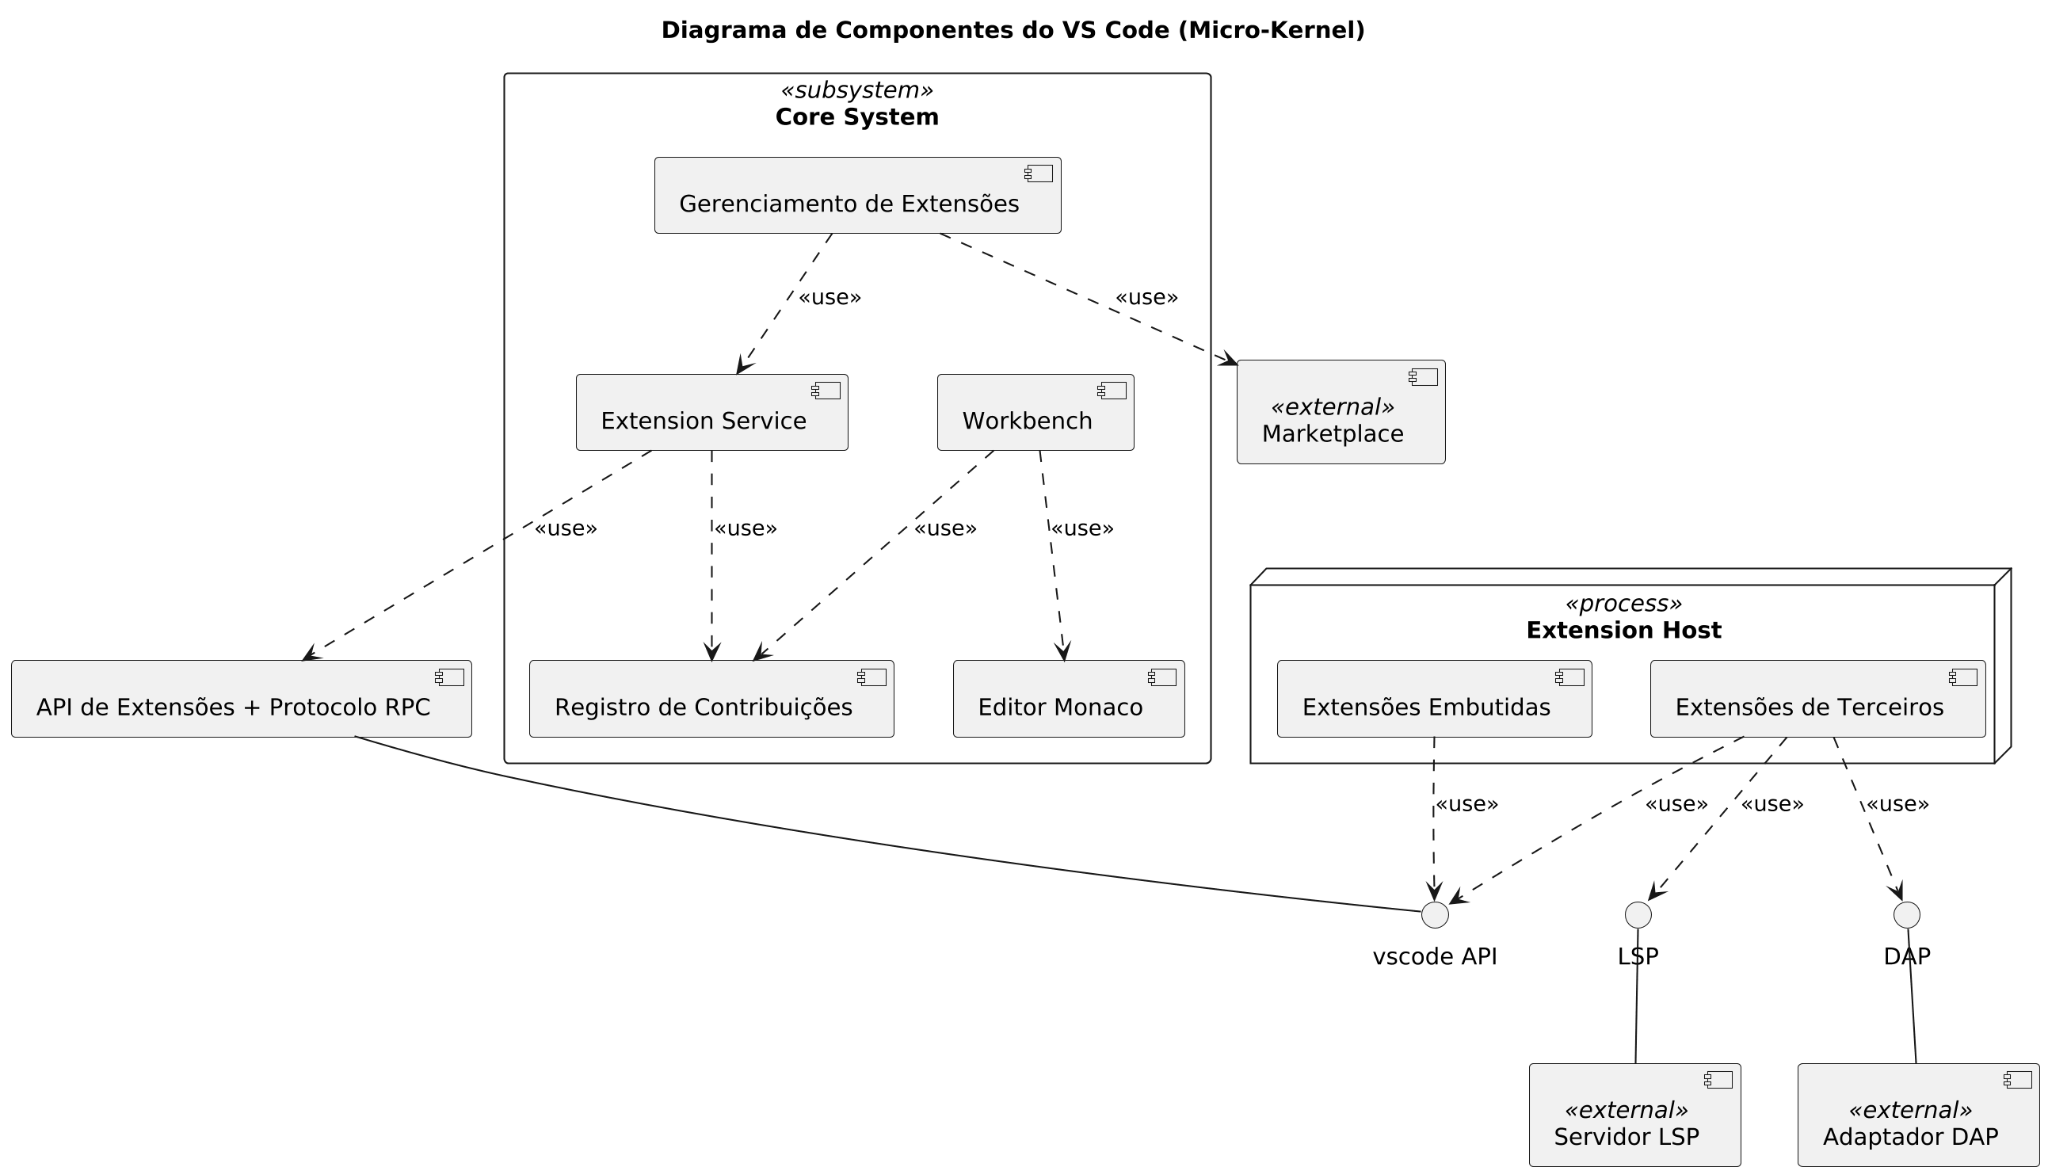
\includegraphics[height=0.75\textheight, keepaspectratio]{vscode_comp.png}
\fonte{Elaboração própria (2026). Componentes mais críticos da orquestração entre núcleo e extensões.}
\end{frame}

\begin{frame}{Visual Studio Code: Diagrama de Módulos}
\centering
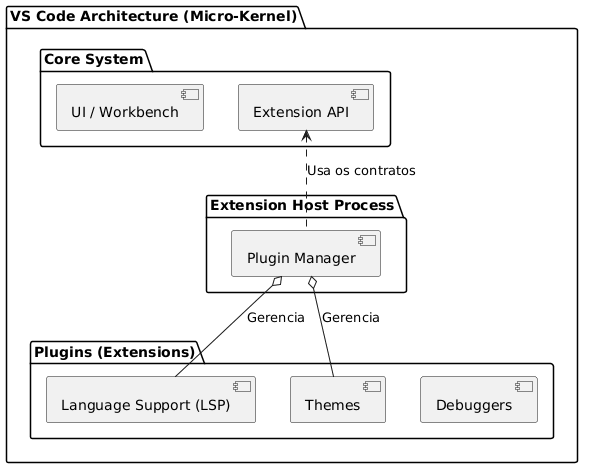
\includegraphics[height=0.75\textheight, keepaspectratio]{vscode_mod.png}
\fonte{Elaboração própria (2026). Isolamento entre interface, gerenciamento de extensões e plugins de terceiros.}
\end{frame}

\begin{frame}{Visual Studio Code: Táticas Arquiteturais (1/2)}
\begin{itemize}\setlength{\itemsep}{0.8em}
\item \textbf{Tática para Extensibilidade e Reuso:}
  \begin{itemize}
  \item Particionamento de componentes (Microkernel) combinado com o particionamento de domínio (LSP).
  \item Permite adicionar extensões sem alterar o núcleo e reaproveitar servidores de linguagem em ferramentas externas.
  \end{itemize}
\item \textbf{Tática para Tolerância a Falhas e Confiabilidade:}
  \begin{itemize}
  \item Isolamento de processos por meio do \textit{Extension Host}.
  \item Evita que \textit{crashes} ou consumo excessivo de CPU por parte de plugins derrubem a interface principal.
  \end{itemize}
\end{itemize}
\end{frame}

\begin{frame}{Visual Studio Code: Táticas Arquiteturais (2/2)}
\begin{itemize}\setlength{\itemsep}{0.8em}
\item \textbf{Tática para Desempenho (\textit{Performance}):}
  \begin{itemize}
  \item Troca de mensagens assíncronas entre o núcleo e os provedores de extensões.
  \item Impede que operações demoradas bloqueiem a \textit{thread} principal de renderização, mantendo a digitação fluida.
  \end{itemize}
\item \textbf{Tática para Agilidade:}
  \begin{itemize}
  \item Forte desacoplamento por meio da padronização da \textit{Extension API}.
  \item Permite a evolução independente do núcleo e do ecossistema, com entregas contínuas e rápidas sem recompilação completa do produto.
  \end{itemize}
\end{itemize}
\end{frame}

% ==========================================================
% OBS STUDIO
% ==========================================================

\begin{frame}{OBS Studio: Características Gerais}
Na análise do OBS Studio, identificaram-se as seguintes características arquiteturais:
\begin{itemize}\setlength{\itemsep}{0.4em}
\item \textbf{Extensibilidade:} Registro padronizado de fontes, codificadores e saídas via \texttt{obs-module.h}.
\item \textbf{Agilidade:} Módulos evoluem de forma independente, mantidos por centenas de colaboradores \textit{open source}.
\item \textbf{Desempenho:} Fundamental para o processamento multimídia em tempo real.
\item \textbf{Confiabilidade e Tolerância a Falhas:} Falhas de rede e de dispositivos de captura não podem travar o núcleo.
\item \textbf{Capacidade de Aprendizado (\textit{Learnability}):} Interface rica e intuitiva para usuários leigos.
\item \textbf{Testabilidade:} O núcleo pode ser testado sem inicializar a interface Qt.
\item \textbf{Implantabilidade e Portabilidade:} Instalações consistentes e independentes em múltiplos SOs.
\end{itemize}
\end{frame}

\begin{frame}{OBS Studio: Principais Características (Top 4) (1/2)}
\begin{itemize}\setlength{\itemsep}{0.8em}
\item \textbf{Extensibilidade (ADR-006):}
  \begin{itemize}
  \item É a razão de ser da arquitetura Microkernel no OBS Studio.
  \item Captura, codificação e saída padrão são entregues como módulos em \texttt{plugins/}, pelo mesmo contrato (\texttt{obs-module.h}) oferecido a terceiros.
  \item Novos codecs, dispositivos e serviços de \textit{streaming} são adicionados sem recompilar o núcleo.
  \end{itemize}
\item \textbf{Desempenho (\textit{Performance}) (ADR-002):}
  \begin{itemize}
  \item A 30 ou 60 quadros por segundo, um quadro perdido é percebido de imediato.
  \item Motivou o núcleo em C, o compartilhamento de texturas na GPU (ADR-IMP-003) e a baixa latência com os plugins de codificação.
  \end{itemize}
\end{itemize}
\end{frame}

\begin{frame}{OBS Studio: Principais Características (Top 4) (2/2)}
\begin{itemize}\setlength{\itemsep}{0.8em}
\item \textbf{Confiabilidade e Tolerância a Falhas (ADR-003):}
  \begin{itemize}
  \item Uma transmissão ao vivo não pode ser repetida, e falhas de rede e de dispositivos são esperadas, não excepcionais.
  \item Isolamento do \textit{loop} de renderização e \textit{threads} próprias para rede e captura, com reconexão automática.
  \end{itemize}
\item \textbf{Implantabilidade e Portabilidade (ADR-005):}
  \begin{itemize}
  \item O software atende usuários de Windows, macOS e Linux e precisa receber novos módulos sem recompilar o núcleo.
  \item Abstração das chamadas nativas, módulos de captura por plataforma (\texttt{win-capture}, \texttt{mac-capture}, \texttt{linux-capture}) e carregamento dinâmico (ADR-IMP-004).
  \end{itemize}
\end{itemize}
\end{frame}

\begin{frame}{OBS Studio: Características Fora do Top 4}
\begin{itemize}\setlength{\itemsep}{0.8em}
\item \textbf{Agilidade:} É, em grande parte, consequência da Extensibilidade: como os módulos evoluem de forma independente, a comunidade entrega mudanças sem alterar o núcleo.
\item \textbf{Testabilidade:} Decorre do desacoplamento que o próprio estilo já exige; é um benefício da estrutura, não sua motivação.
\item \textbf{Capacidade de Aprendizado:} É resolvida na camada de interface (Qt), que pode ser substituída sem afetar o motor, e por isso não determina a estrutura de componentes.
\end{itemize}
\end{frame}

\begin{frame}{OBS Studio: Decisões Arquiteturais (ADRs) (1/2)}
\begin{itemize}\setlength{\itemsep}{0.8em}
\item \textbf{ADR-IMP-001: Adoção da Linguagem C para o Núcleo}
  \begin{itemize}
  \item \textbf{Decisão:} Desenvolver o núcleo \texttt{libobs} em C, em vez de C++ ou de outra linguagem de mais alto nível.
  \item \textbf{Consequências:} Garante latência mínima e uma Interface Binária de Aplicação (ABI) estável, à qual plugins e interfaces escritos em outras linguagens podem se ligar.
  \end{itemize}
\item \textbf{ADR-IMP-002: Desacoplamento da Interface Visual por meio do framework Qt}
  \begin{itemize}
  \item \textbf{Decisão:} Isolar a interface em C++ com o framework Qt, comunicando-se com o núcleo apenas pela API exportada (\texttt{obs.h}).
  \item \textbf{Consequências:} Evita lógica visual nas camadas multimídia; a interface pode ser substituída e clientes alternativos podem ser construídos.
  \end{itemize}
\end{itemize}
\end{frame}

\begin{frame}{OBS Studio: Decisões Arquiteturais (ADRs) (2/2)}
\begin{itemize}\setlength{\itemsep}{0.8em}
\item \textbf{ADR-IMP-003: Compartilhamento de Contexto Gráfico (\textit{Zero-Copy})}
  \begin{itemize}
  \item \textbf{Decisão:} Os plugins trocam apenas referências a texturas armazenadas na memória da GPU, sem copiar os pixels.
  \item \textbf{Consequências:} Reduz o uso de CPU e de RAM; em contrapartida, plugins visuais precisam executar nas \textit{threads} gráficas controladas pelo OBS.
  \end{itemize}
\item \textbf{ADR-IMP-004: Injeção de Funcionalidades via Carregamento Dinâmico}
  \begin{itemize}
  \item \textbf{Decisão:} Utilizar as APIs nativas de carregamento dinâmico de bibliotecas de cada sistema operacional durante a inicialização.
  \item \textbf{Consequências:} Arquitetura \textit{plug and play}: o núcleo varre as pastas de plugins, carrega as bibliotecas e registra os \textit{callbacks} de cada módulo.
  \end{itemize}
\end{itemize}
\end{frame}

\begin{frame}{OBS Studio: Componentes do Sistema Central}
\begin{itemize}\setlength{\itemsep}{0.65em}
\item \textbf{Microkernel (\texttt{libobs}):} Orquestra o \textit{pipeline} multimídia, sincroniza as faixas de áudio e vídeo em tempo real, gerencia o ciclo de vida da aplicação e carrega e descarrega os plugins em tempo de execução.
\item \textbf{Plugin Interface (\texttt{obs-module}):} Cabeçalhos C que definem como um plugin se registra, declara suas capacidades e se comunica com o \texttt{libobs}.
\item \textbf{Interface do Usuário (Qt Frontend):} Painel de controle visual e intuitivo que atua como um cliente externo, enviando comandos ao núcleo.
\end{itemize}
\end{frame}

\begin{frame}{OBS Studio: Componentes Periféricos (Plugins)}
\begin{itemize}\setlength{\itemsep}{0.65em}
\item \textbf{Plugins de Fontes (\textit{Source Plugins}):} Capturam dados brutos de dispositivos (câmeras e microfones) ou de janelas do sistema operacional.
\item \textbf{Plugins de Codificação (\textit{Encoder Plugins}):} Recebem os quadros compostos pelo núcleo e aplicam compressão apoiada pelas APIs das placas gráficas.
\item \textbf{Plugins de Saída (\textit{Output Plugins}):} Módulos assíncronos que empacotam e enviam o vídeo pela rede (ex.: RTMP) ou o gravam em disco, reconectando-se em caso de falha.
\end{itemize}
\end{frame}

\begin{frame}{OBS Studio: Diagrama de Componentes}
\centering
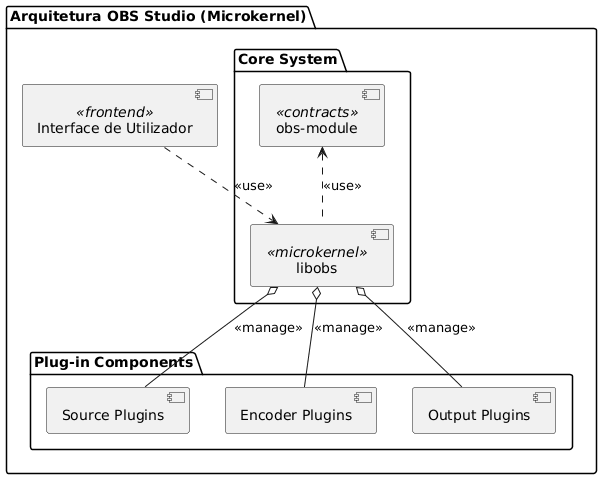
\includegraphics[height=0.75\textheight, keepaspectratio]{obs_comp.png}
\fonte{Elaboração própria (2026). Fluxo essencial: Captura $\rightarrow$ Núcleo $\rightarrow$ Compressão $\rightarrow$ Saída.}
\end{frame}

\begin{frame}{OBS Studio: Diagrama de Módulos}
\centering
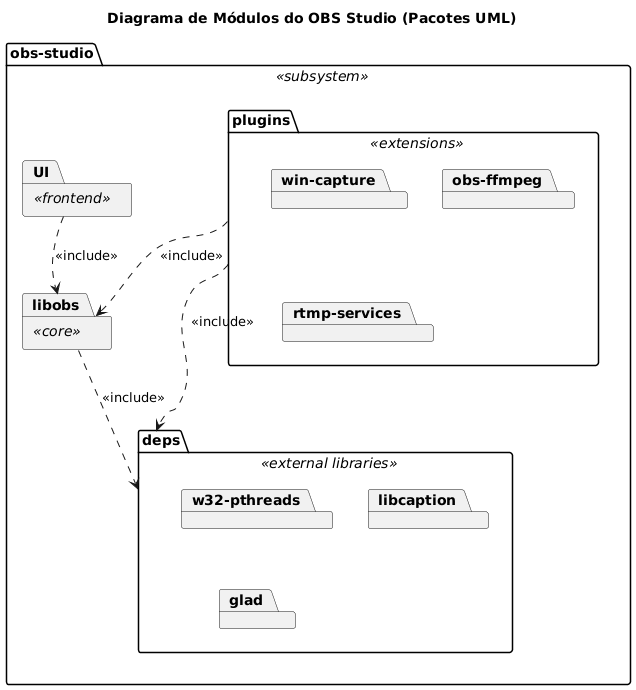
\includegraphics[height=0.75\textheight, keepaspectratio]{obs_mod.png}
\fonte{Elaboração própria (2026). Isolamento prático das bibliotecas e interfaces em pacotes.}
\end{frame}

\begin{frame}{OBS Studio: Táticas Arquiteturais (1/2)}
\begin{itemize}\setlength{\itemsep}{0.8em}
\item \textbf{Tática para Implantabilidade:}
  \begin{itemize}
  \item \textit{Binding} em tempo de execução para descobrir e carregar os plugins, facilitando instaladores independentes e a atualização modular sem recompilar o núcleo.
  \end{itemize}
\item \textbf{Tática para Desempenho (\textit{Performance}):}
  \begin{itemize}
  \item Aumento da eficiência de recursos com operações \textit{zero-copy} e aceleração por hardware, compartilhando texturas diretamente na GPU.
  \end{itemize}
\item \textbf{Tática para Confiabilidade e Tolerância a Falhas:}
  \begin{itemize}
  \item Execução assíncrona de rede e captura em \textit{threads} separadas e tratamento local de erros, impedindo que falhas congelem o \textit{loop} de renderização ou encerrem a aplicação.
  \end{itemize}
\end{itemize}
\end{frame}

\begin{frame}{OBS Studio: Táticas Arquiteturais (2/2)}
\begin{itemize}\setlength{\itemsep}{0.55em}
\item \textbf{Tática para Extensibilidade:}
  \begin{itemize}
  \item Registro padronizado via \texttt{obs-module.h}: cada plugin declara, em \texttt{obs\_module\_load()}, as fontes, os codificadores e as saídas que oferece.
  \end{itemize}
\item \textbf{Tática para Agilidade:}
  \begin{itemize}
  \item Encapsulamento e interfaces padronizadas criam fronteiras rígidas, permitindo que a comunidade integre plugins sem risco ao núcleo.
  \end{itemize}
\item \textbf{Tática para Testabilidade:}
  \begin{itemize}
  \item Abstração de interfaces (\texttt{libobs} separado do Qt), permitindo simular e testar o núcleo sem inicializar a interface gráfica.
  \end{itemize}
\item \textbf{Tática para Capacidade de Aprendizado:}
  \begin{itemize}
  \item Separação da interface em Qt, com o Modo Estúdio e \textit{feedback} visual que reduzem a curva de aprendizado.
  \end{itemize}
\end{itemize}
\end{frame}

% ==========================================================
% CONCLUSÃO
% ==========================================================

\begin{frame}{Conclusão e Aprendizados}
\begin{itemize}\setlength{\itemsep}{0.6em}
\item A arquitetura \textbf{Microkernel} mostrou-se adequada para isolar a coordenação central, permitindo que ecossistemas extensos evoluam em paralelo de forma sustentável.
\item No \textbf{Visual Studio Code}, o foco foi a proteção contra plugins defeituosos, por meio do isolamento de processos (\textit{Extension Host}), e a ativação sob demanda.
\item No \textbf{OBS Studio}, as decisões priorizaram o desempenho em tempo real, com um núcleo de baixa latência em C e otimização \textit{zero-copy} na GPU.
\item \textbf{Contraste:} No VS Code, os plugins rodam em outro processo; no OBS, rodam no mesmo processo do núcleo, e a proteção vem de \textit{threads} separadas e do tratamento local de erros.
\item \textbf{O Pilar Central:} Em ambos os sistemas, contratos e APIs rigorosos (as regras de fronteira) foram decisivos para garantir a agilidade e impedir o colapso estrutural.
\end{itemize}
\end{frame}

\begin{frame}{Referências}
\scriptsize
\begin{itemize}\setlength{\itemsep}{0.3em}
\item RICHARDS, M.; FORD, N. \textbf{Fundamentals of Software Architecture}: An Engineering Approach. 1. ed. Sebastopol: O'Reilly Media, 2020.
\item MICROSOFT. \textbf{Extension Host}. Disponível em: \url{https://code.visualstudio.com/api/advanced-topics/extension-host}. Acesso em: 29 set. 2026.
\item MICROSOFT. \textbf{Activation Events}. Disponível em: \url{https://code.visualstudio.com/api/references/activation-events}. Acesso em: 29 set. 2026.
\item MICROSOFT. \textbf{Language Server Protocol}. Disponível em: \url{https://microsoft.github.io/language-server-protocol/}. Acesso em: 29 set. 2026.
\item MICROSOFT. \textbf{Workspace Trust}. Disponível em: \url{https://code.visualstudio.com/docs/editing/workspace-trust}. Acesso em: 29 set. 2026.
\item MICROSOFT. \textbf{Visual Studio Code}. Repositório no GitHub. Disponível em: \url{https://github.com/microsoft/vscode}. Acesso em: 29 set. 2026.
\item OBS PROJECT. \textbf{Backend Design}. Disponível em: \url{https://docs.obsproject.com/backend-design}. Acesso em: 29 set. 2026.
\item OBS PROJECT. \textbf{Plugins}. Disponível em: \url{https://docs.obsproject.com/plugins}. Acesso em: 29 set. 2026.
\item OBS PROJECT. \textbf{OBS Studio}. Repositório no GitHub. Disponível em: \url{https://github.com/obsproject/obs-studio}. Acesso em: 29 set. 2026.
\end{itemize}
\end{frame}

\begin{frame}[plain,c,noframenumbering]
\begin{center}
\Huge \textbf{Obrigado!} \\
\vspace{1cm}
\Large Perguntas e Comentários
\end{center}
\end{frame}

\end{document}